Coloca en orden de menor a mayor los siguientes colores, de acuerdo con el valor de su frecuencia (de izquierda a derecha).
\begin{center}
    \ifprintanswers
        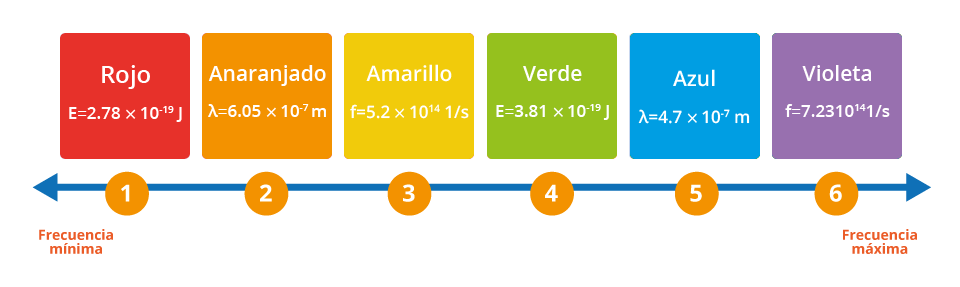
\includegraphics[width=0.9\textwidth ]{../images/SINFI_U3_AC76_IMG1a}
    \else
        \dashedbox{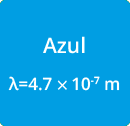
\includegraphics[width=0.1\textwidth ]{../images/SINFI_U3_AC76_IMG6_462446}} \qquad
        \dashedbox{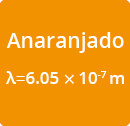
\includegraphics[width=0.1\textwidth ]{../images/SINFI_U3_AC76_IMG3}} \qquad
        \dashedbox{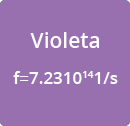
\includegraphics[width=0.1\textwidth ]{../images/SINFI_U3_AC76_IMG7}} \qquad
        \dashedbox{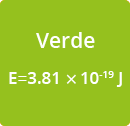
\includegraphics[width=0.1\textwidth ]{../images/SINFI_U3_AC76_IMG5_739556}} \qquad
        \dashedbox{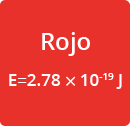
\includegraphics[width=0.1\textwidth ]{../images/SINFI_U3_AC76_IMG2}} \qquad
        \dashedbox{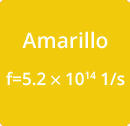
\includegraphics[width=0.1\textwidth ]{../images/SINFI_U3_AC76_IMG4}} \qquad
        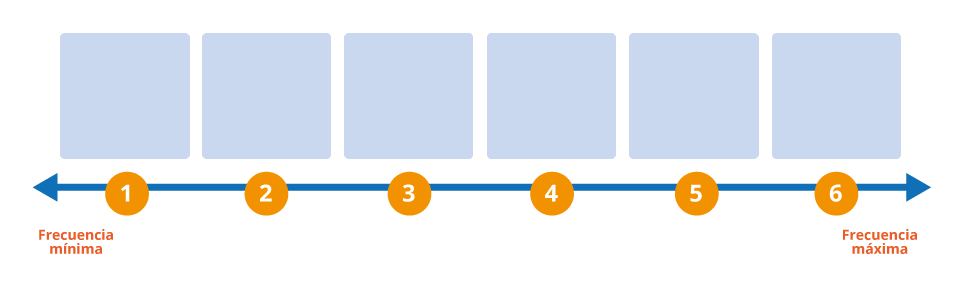
\includegraphics[width=0.9\textwidth ]{../images/SINFI_U3_AC76_IMG1}
    \fi
\end{center}
